\documentclass{article}
\usepackage{graphicx} % Required for inserting images
\usepackage{amsmath, amssymb} % For \text in math mode and \mathbb

\title{NLP hw2}
\author{Tamar Tabbach, Gal Barak, Adam Fleisher}
\date{May 2026}

\begin{document}

\maketitle

\section{Word-Level Neural Bi-gram Language Model}

\subsection*{(a)}
\textbf{Step 1: Simplifying the Cross Entropy Function}

First, we substitute the definition of the softmax function into the Cross Entropy loss and apply logarithm rules:

$$\text{CE}(\mathbf{y}, \hat{\mathbf{y}}) = -\sum_i y_i \log(\hat{y}_i)$$

$$= -\sum_i y_i \log\left( \frac{\exp(\theta_i)}{\sum_j \exp(\theta_j)} \right)$$

$$= -\sum_i y_i \left( \log(\exp(\theta_i)) - \log\left(\sum_j \exp(\theta_j)\right) \right)$$

Since $\log(\exp(x)) = x$, we get:

$$= -\sum_i y_i \left( \theta_i - \log\left(\sum_j \exp(\theta_j)\right) \right)$$

\vspace{1em}
\textbf{Step 2: Differentiating with respect to } $\theta_k$

Now we take the partial derivative with respect to $\theta_k$:

$$\frac{\partial \text{CE}}{\partial \theta_k} = -\frac{\partial}{\partial \theta_k} \left[ \sum_i y_i \theta_i - \sum_i y_i \log\left(\sum_j \exp(\theta_j)\right) \right]$$

$$= -\left[ y_k \cdot 1 - \sum_i y_i \cdot \frac{\partial}{\partial \theta_k} \log\left(\sum_j \exp(\theta_j)\right) \right]$$

Using the chain rule for the logarithm term:

$$= -\left[ y_k - \sum_i y_i \cdot \frac{\exp(\theta_k)}{\sum_j \exp(\theta_j)} \right]$$

We can pull out the term that does not depend on $i$:

$$= -y_k + \left( \sum_i y_i \right) \frac{\exp(\theta_k)}{\sum_j \exp(\theta_j)}$$

Since $\mathbf{y}$ is a one-hot vector, the sum of its elements is 1 (i.e., $\sum_i y_i = 1$). Additionally, by definition, $\frac{\exp(\theta_k)}{\sum_j \exp(\theta_j)} = \hat{y}_k$. Substituting these back yields the final result:

$$= -y_k + 1 \cdot \hat{y}_k = \hat{y}_k - y_k$$

\subsection*{(b)}
\textbf{Step 1: Applying the Chain Rule}

To find the gradient of the loss $J$ with respect to the input $\mathbf{x}$, we use the chain rule. First, let us define the intermediate variables of the network:
\begin{align*}
    \mathbf{z}_1 &= \mathbf{x}\mathbf{W}_1 + \mathbf{b}_1 \\
    \mathbf{h} &= \sigma(\mathbf{z}_1) \\
    \mathbf{z}_2 &= \mathbf{h}\mathbf{W}_2 + \mathbf{b}_2 \\
    \hat{\mathbf{y}} &= \text{softmax}(\mathbf{z}_2)
\end{align*}

The chain rule backward from the loss $J$ to the input $\mathbf{x}$ is given by:
$$\frac{\partial J}{\partial \mathbf{x}} = \frac{\partial J}{\partial \mathbf{z}_2} \cdot \frac{\partial \mathbf{z}_2}{\partial \mathbf{h}} \cdot \frac{\partial \mathbf{h}}{\partial \mathbf{z}_1} \cdot \frac{\partial \mathbf{z}_1}{\partial \mathbf{x}}$$

\vspace{1em}
\textbf{Step 2: Calculating Individual Derivatives}

Now, we compute each component in the chain separately:
\begin{itemize}
    \item $\frac{\partial \mathbf{z}_1}{\partial \mathbf{x}} = \mathbf{W}_1^T$ (Derivative of the first linear transformation)
    \item $\frac{\partial \mathbf{h}}{\partial \mathbf{z}_1}$ represents the derivative of the sigmoid function. It is structured as a $D_h \times D_h$ diagonal Jacobian matrix where the elements on the main diagonal are the derivatives of each individual activation $h_i$, and all off-diagonal elements are zero:
    $$ \begin{pmatrix}
    h_1(1-h_1) & 0 & \cdots & 0 \\
    0 & h_2(1-h_2) & \cdots & 0 \\
    \vdots & \vdots & \ddots & \vdots \\
    0 & 0 & \cdots & h_{D_h}(1-h_{D_h})
    \end{pmatrix} $$
    \item $\frac{\partial \mathbf{z}_2}{\partial \mathbf{h}} = \mathbf{W}_2^T$ (Derivative of the second linear transformation)
    \item $\frac{\partial J}{\partial \mathbf{z}_2} = \hat{\mathbf{y}} - \mathbf{y}$ (This is the gradient of the Cross Entropy loss with respect to the input of the softmax function, which was already derived in section a)
\end{itemize}

\vspace{1em}
\textbf{Step 3: The Final Result}

Multiplying all the terms together from left to right, we get the final gradient:

$$ \frac{\partial J}{\partial \mathbf{x}} = (\hat{\mathbf{y}} - \mathbf{y}) \mathbf{W}_2^T \begin{pmatrix}
h_1(1-h_1) & 0 & \cdots & 0 \\
0 & h_2(1-h_2) & \cdots & 0 \\
\vdots & \vdots & \ddots & \vdots \\
0 & 0 & \cdots & h_{D_h}(1-h_{D_h})
\end{pmatrix} \mathbf{W}_1^T $$

\subsection*{(d)}

Based on the training iterations of the neural bi-gram language model using GloVe embeddings, the final evaluation yielded the following result:

\begin{itemize}
    \item \textbf{Dev Perplexity:} 112.8621
\end{itemize}

\vspace{0.5em}
\noindent \textit{Note: The trained parameters have been saved to \texttt{saved\_params\_40000.npy} and are included in the submission zip file.}

\newpage
\section{Generating Shakespeare with a Char-level LM}
\subsection*{(a)}
Character-based models easily handle out-of-vocabulary words and misspellings by building them character by character, and they require far fewer embedding parameters. Meanwhile, word-based models capture semantic meaning and contextual relationships more naturally. Additionally, word-based models yield shorter sequences, reducing computational costs and making it easier for the network to learn long-range dependencies without forgetting past context.
\subsection*{(c)}
\begin{figure}[h]
    \centering
    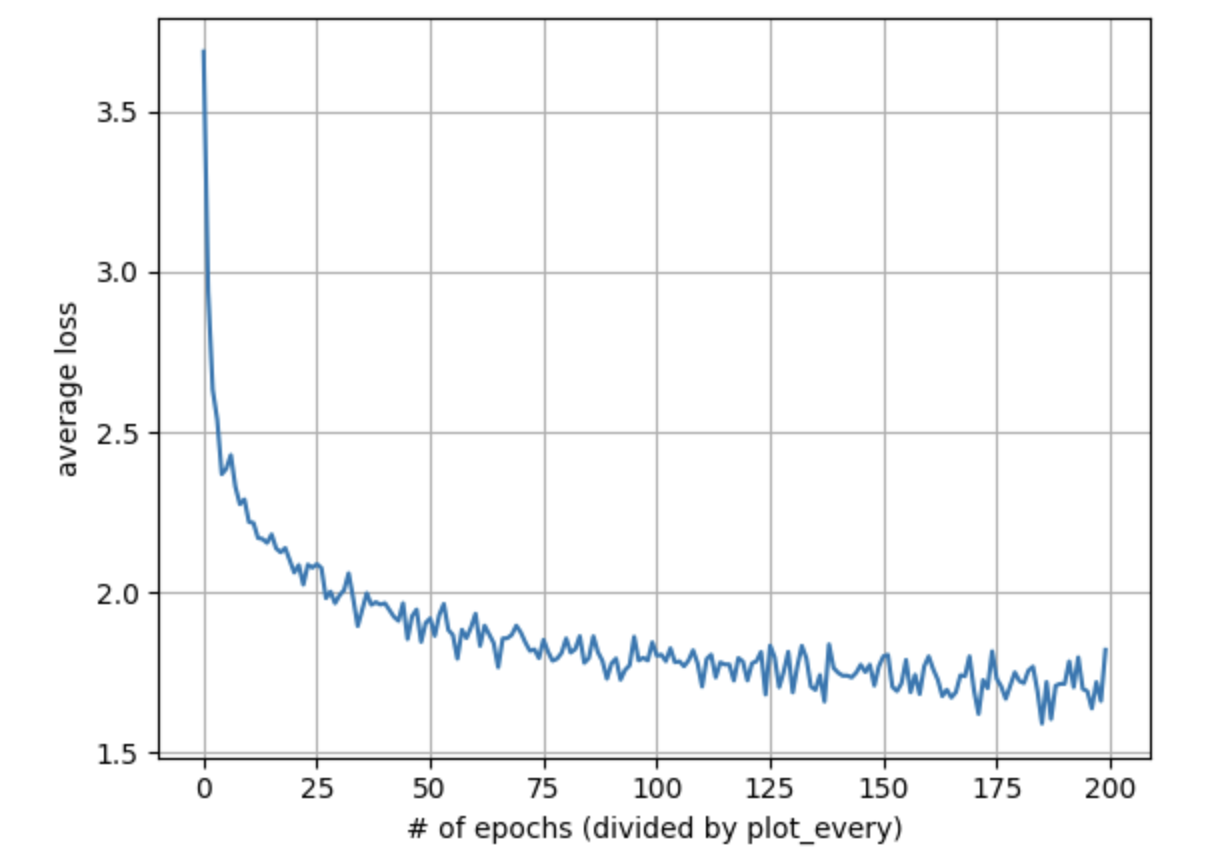
\includegraphics[width=0.75\linewidth]{q2c_loss_curve.png}
    \caption{Training loss curve for the character-level Shakespeare language model: average loss versus training-step index, where each tick on the x-axis corresponds to \texttt{plot\_every} SGD iterations.}
    \label{fig:q2c_loss_curve}
\end{figure}

\newpage
\section{Perplexity}
\subsection*{(a)}

Let $x_i = p(s_{i}|s_{1},...,s_{i-1})$ represent the conditional probability of token $s_i$. We begin with the left-hand side of the perplexity equation:

\[
2^{-\frac{1}{M}\sum_{i=1}^{M}\log_{2}x_i}
\]

Using the algebraic property of exponents where $a^{B \cdot C} = (a^B)^C$, we can isolate the summation term from the outer scaling factor:

\[
= \left( 2^{\sum_{i=1}^{M}\log_{2}x_i} \right)^{-\frac{1}{M}}
\]

Next, using the exponent property where a sum in the exponent translates to a product of bases ($a^{\sum z_i} = \prod a^{z_i}$), we can rewrite the inner expression as:

\[
= \left( \prod_{i=1}^{M} 2^{\log_2 x_i} \right)^{-\frac{1}{M}}
\]

Since $2^{\log_2 x_i} = x_i$, the terms inside the product simplify directly to the joint probability components:

\[
= \left( \prod_{i=1}^{M} x_i \right)^{-\frac{1}{M}}
\]

Next, using the natural logarithm identity, we can express each probability term $x_i$ in base $e$ as $x_i = e^{\ln x_i}$:

\[
= \left( \prod_{i=1}^{M} e^{\ln x_i} \right)^{-\frac{1}{M}}
\]

When multiplying terms with identical bases, we add their exponents together ($\prod e^{z_i} = e^{\sum z_i}$), turning the product back into a summation in the exponent of $e$:

\[
= \left( e^{\sum_{i=1}^{M} \ln x_i} \right)^{-\frac{1}{M}}
\]

Finally, by applying the power-of-a-power exponent rule once more, we multiply the inner and outer exponents:

\[
= e^{-\frac{1}{M}\sum_{i=1}^{M}\ln x_i}
\]

Substituting $x_i = p(s_{i}|s_{1},...,s_{i-1})$ back into the formula gives us the right-hand side of the equation:

\[
= e^{-\frac{1}{M}\sum_{i=1}^{M}\ln p(s_{i}|s_{1},...,s_{i-1})}
\]

This completes the proof, showing that both expressions are mathematically identical.

\subsection*{(b)}

\begin{table}[h]
    \centering
    \begin{tabular}{lcc}
        \hline
        Model-Data & Wikipedia Text & Shakespearean Text \\
        \hline
        Word-Level Neural Bi-gram (Section 1) & 72.40 & 125.68 \\
        Character-level RNN (Section 2)       & 16.19 & 7.09   \\
        \hline
    \end{tabular}
    \caption{Perplexity of the two trained language models on the Wikipedia and Shakespearean passages. Word-level perplexity is per-token; character-level perplexity is per-character, so numbers are not directly comparable across rows.}
    \label{tab:q3b_perplexity}
\end{table}

\subsection*{(c)}

The main factor within each row is train/test domain match. The word-level bigram was trained on Penn Treebank (modern English), so it scores far better on Wikipedia (72.40) than on Shakespeare (125.68), where archaic syntax and rare word-to-word transitions are poorly modeled by a bigram trained on modern English. The character-level RNN shows the opposite pattern, modeling its in-domain Shakespeare (7.09) more confidently than the unfamiliar Wikipedia text (16.19). The large gap \emph{between} rows is mostly an artifact of granularity, not quality: word-level perplexity is per-token over a 2000-word vocabulary, whereas character-level perplexity is per-character over a 100-symbol alphabet, giving a much smaller branching factor. The two rows therefore measure uncertainty over different units and are only directly comparable within a row.

\newpage
\section{Implementing a Transformer Model}
\subsection*{(a)}

Multi-head attention splits each token's $d_{model}$-dimensional vector across $N_h$ (num\_heads) heads of size $d_k = d_{model} / N_h$, then concatenates the per-head outputs and reshapes them back to $d_{model}$. This requires $N_h \cdot d_k = d_{model}$. The assertion $d_{model} \bmod N_h = 0$ enforces this: otherwise the integer division $\lfloor d_{model} / N_h \rfloor$ discards a remainder, the concatenated dimension is smaller than $d_{model}$, and the final reshape back to $d_{model}$ fails. Checking it in the constructor catches the error at construction rather than as a confusing crash inside the forward pass.

\subsection*{(b)}

\noindent\textbf{(i) Architecture changes.} BERT is encoder-only, operating on a single sequence. We therefore \emph{remove} the decoder stack, the cross-attention sub-layer (which only existed to bridge target to source), and the separate decoder embedding; we \emph{keep} the encoder stack, a single token embedding, and the positional encoding. The prediction head (final linear layer to vocabulary logits) is moved onto the encoder output, producing one distribution per input position, and the cross-entropy loss is applied \emph{only at the masked positions}.

\medskip

\noindent\textbf{(ii) Masking strategy.} The two masks change in opposite directions. The attention (no-peek) mask is \emph{removed}: it enforced the autoregressive constraint that position $t$ cannot see the future, but BERT needs \emph{bidirectional} context, so self-attention runs fully unmasked. In its place we \emph{add} token-level masking (absent from the autoregressive model): roughly 15\% of input tokens are replaced with a \texttt{[MASK]} token before embedding, and the model is trained to reconstruct the originals at those positions. In short, the autoregressive model masks in \emph{attention} and leaves the input intact, whereas the MLM uses no attention mask but corrupts the \emph{input}.

\newpage
\section{Attention Exploration}
\subsection*{1.Copying in attention:}
\subsubsection*{(a)}
$\alpha$ can be interpreted as a categorical probability distribution since:
\begin{enumerate}
    \item $\forall i\in[n]\  \alpha_i=\frac{\exp(k_i^\top q)}{\sum_{j=1}^n\exp(k_j^\top q)}\ge0$, since $\exp(x)>0 \ \forall x\in \mathbb{R}$.
    \item $\sum_{i=1}^n\alpha_i=\sum_{i=1}^n\frac{\exp(k_i^\top q)}{\sum_{j=1}^n\exp(k_j^\top q)}=\frac{1}{\sum_{j=1}^n\exp(k_j^\top q)}\sum_{i=1}^n\exp(k_i^\top q)=1$.
\end{enumerate}
Therefore it satisfies both of the conditions required to be a categorical probability distribution.

\subsubsection*{(b)}
This happens when $k_j$ is much more aligned with the query $q$ than all other keys, i.e.:
\[
k_j^\top q \gg k_i^\top q \quad \forall i\neq j.
\]
\subsubsection*{(c)}
Under the conditions described above, we have $\alpha_j \approx 1$ and $\alpha_i \approx 0$ for all $i \neq j$. Therefore,
\[
c = \sum_{i=1}^n \alpha_i v_i \approx v_j.
\]
Thus, the attention output is approximately the value vector corresponding to the dominant key.

\subsubsection*{(d)}
Together, this means that when the query is much more aligned with one key than with the others, the attention mechanism assigns almost all probability mass to the corresponding value vector, effectively copying it to the output.

\newpage
\subsection*{2.An average of two:}
\subsubsection*{(a)}
First let us solve the hint by defining:
\[
A_i = a_i a_i^\top .
\]
Since $\lVert a_i \rVert = 1$, we have:
\[
A_i a_i = (a_i a_i^\top) a_i = a_i(a_i^\top a_i)=a_i \lVert a_i \rVert^2 = a_i.
\]
Moreover, for every vector $b$ s.t. $b^\top a_i=0$:
\[
A_i b = (a_i a_i^\top) b = a_i(a_i^\top b)=0.
\]
Thus, $A_i$ projects onto the direction spanned by $a_i$.
Now we define:
\[
M:=\sum_{i=1}^mA_i=\sum_{i=1}^m a_i a_i^\top .
\]
Let there be some vector $s=v_a+v_b, \ s.t \ v_a\in A, \ v_b\in B$. Therefore there exists
some $\lambda_1,...\lambda_m, \gamma_1,...\gamma_p$ s.t.:
\[
v_a=\sum_{i=1}^m\lambda_ia_i,\ \ v_b=\sum_{i=1}^p\gamma_ib_i
\]
So:
\[
Ms=M(v_a+v_b)=Mv_a+Mv_b=\sum_{i=1}^mA_i\sum_{j=1}^m\lambda_ja_j+\sum_{i=1}^mA_i\sum_{j=1}^p\gamma_jb_j
\]
\[
\sum_{i=1}^mA_i\sum_{j=1}^m\lambda_ja_j=\sum_{i=1}^m\sum_{j=1}^m\lambda_jA_ia_j 
\]
From previous proof $A_i a_j = a_i$ if $i=j$, and $A_i a_j=0$ otherwise (since this is an orthonormal basis), therefore:
\[
\sum_{i=1}^mA_i\sum_{j=1}^m\lambda_ja_j= \sum_{i=1}^m\lambda_ia_i=v_a.
\]
Similarly $A_ib_j=0\forall i\in[m], j\in[p]$ because $a_i^\top b_j=0$ by orthogonality of $A$ and $B$:
\[
\sum_{i=1}^mA_i\sum_{j=1}^p\gamma_jb_j=\sum_{i=1}^m\sum_{j=1}^p\gamma_jA_ib_j=0
\]
So we conclude $Ms=v_a$ as required.

\subsubsection*{(b)}

Let us define:
\[
q=\lambda(k_a+k_b),
\]
where $\lambda>0$ is a large scalar. Since the key vectors are orthogonal and have unit norm, we get
\[
k_a^\top q=\lambda,\qquad k_b^\top q=\lambda,
\]
and for every $i\neq a,b$,
\[
k_i^\top q=0.
\]
Therefore, the softmax assigns equal attention weights to $v_a$ and $v_b$, and much smaller weights to all other value vectors:
\[
\alpha_a=\alpha_b=\frac{e^\lambda}{2e^\lambda+(n-2)} \approx \frac{1}{2},
\qquad
\alpha_i=\frac{1}{2e^\lambda+(n-2)}\approx 0
\quad \text{for } i\neq a,b.
\]
Hence,
\[
c=\sum_{i=1}^n \alpha_i v_i \approx \frac{1}{2}(v_a+v_b).
\]

\newpage
\subsection*{3.Drawbacks of single-headed attention:}
\subsubsection*{(a)}
Since $\Sigma_i=\alpha I$ for all $i$ and $\alpha$ is vanishingly small, each sampled key $k_i$ is very close to its mean $\mu_i$. Therefore, we define:
\[
q=\lambda(\mu_a+\mu_b),
\]
Similarly to the previous part. Since the means are orthogonal and have unit norm, we get
\[
\mu_a^\top q=\lambda,\qquad \mu_b^\top q=\lambda,
\]
and for every $i\neq a,b$,
\[
\mu_i^\top q=0.
\]
Because $k_i\approx \mu_i$, it follows that
\[
k_a^\top q\approx \lambda,\qquad k_b^\top q\approx \lambda,\qquad k_i^\top q\approx 0 \quad \text{for } i\neq a,b.
\]
Thus, for sufficiently large $\lambda$, the softmax assigns approximately equal weight to $v_a$ and $v_b$, and negligible weight to the other values:
\[
\alpha_a\approx \alpha_b\approx \frac{1}{2},\qquad \alpha_i\approx 0 \quad \text{for } i\neq a,b.
\]
Hence,
\[
c=\sum_{i=1}^n \alpha_i v_i \approx \frac{1}{2}(v_a+v_b).
\]

\subsubsection*{(b)}
Using the query:
\[
q=\lambda(\mu_a+\mu_b),
\]
and the fact that the variances of the other keys remain as in the previous part we still get:
\[
k_b^\top q\approx\lambda,\qquad k_i^\top q\approx0\ \forall i\notin\{a,b\}
\]
But since the variance of $k_a$ has now changed in a way that roughly preserves the direction of $\mu_a$ but not the norm we get:
\[
k_a^\top q\approx\lambda\lVert k_a\rVert
\]
Which can vary significantly across samples. Since the softmax function is sensitive to such score changes,
the weight $\alpha_a$ may sometimes dominate and sometimes be much smaller.
Therefore, the output $c$ will have high variance across samples and will not reliably satisfy:
\[
c\approx\frac{1}{2}(v_a+v_b)
\]


\newpage
\subsection*{4.Benefits of multi-headed attention:}
\subsubsection*{(a)}
Let us define two different query vectors:
\[
q_1=\lambda \mu_a,\qquad q_2=\lambda \mu_b,
\]
where $\lambda>0$ is a large scalar. Since $\Sigma_i=\alpha I$ with vanishingly small $\alpha$, we have $k_i\approx \mu_i$. Therefore, the first head assigns almost all of its weight to $v_a$, so
\[
c_1\approx v_a,
\]
while the second head assigns almost all of its weight to $v_b$, so
\[
c_2\approx v_b.
\]
Thus, the final multi-headed attention output is
\[
\frac{1}{2}(c_1+c_2)\approx \frac{1}{2}(v_a+v_b).
\]

\subsubsection*{(b)}
Using the queries from the previous part:
\[
q_1=\lambda\mu_a,\qquad q_2=\lambda\mu_b,
\]
The first head is intended to attend to $v_a$, while the second head is intended to attend to $v_b$. Since $k_a$ may have large variance in its norm, the score $k_a^\top q_1$ may vary across samples, and therefore $c_1$ may have some variance.

However, this variation does not strongly affect the second head, since
\[
k_a^\top q_2 \approx \lambda \mu_a^\top \mu_b = 0,
\]
while
\[
k_b^\top q_2 \approx \lambda.
\]
Thus, $c_2\approx v_b$ remains relatively stable. Therefore, the final output
\[
\frac{1}{2}(c_1+c_2)
\]
has lower variance than in the single-headed case, because $v_a$ and $v_b$ do not compete within the same softmax distribution. In the single-head case, if $k_a^\top q$ becomes very large, then the softmax denominator also becomes very large, reducing the relative attention weight assigned to $v_b$. Thus, $v_a$ and $v_b$ directly compete within the same attention distribution. Hence, the multi-headed output is more stable and remains closer to
\[
\frac{1}{2}(v_a+v_b).
\]
\section{AI Disclosure \& Reflection}

\subsection*{(a)}
We have used Gemini web UI, and Claude Code.

\subsection*{(b)}
We have used Gemini for theoretical validation, handwriting to latex conversion, and rephrasing our text. We've used Claude Code for help implementing the Transformer notebook (the multi-head attention, the encoder and decoder layers, and the no-peek mask), computing the perplexities, and drafting parts of the written solution.

\subsection*{(c)}
Only helped, but we mainly used it for things we know how to do to accelerate things, so no surprise noted here.

\end{document}
 